\documentclass[a4paper,11pt]{article}
\usepackage[utf8]{inputenc}
\usepackage[T1]{fontenc}
\usepackage[polish]{babel}
\usepackage{amsmath}
\usepackage{amssymb}
\usepackage{geometry}
\usepackage{graphicx}
\usepackage{multicol}
\geometry{top=0.5in, bottom=0.8in, left=0.8in, right=0.8in}

% Customizable parameters
% Wstaw pełny tytuł zadania
\newcommand{\tasktitle}{Dostawa Piwa}
% Wstaw skrócony tytuł zadania
\newcommand{\taskshort}{PIW}
% Wstaw informacje o konkursie
\newcommand{\contestinfo}{Konkurs Świąteczny 2024 - Grupa Początkująca.}
% Wstaw limit pamięci
\newcommand{\memorylimit}{256 MB}
% Wstaw dane przykładowe wejścia
\newcommand{\exampleinput}{5 20\\4\\8\\7\\3\\6}
% Wstaw dane przykładowe wyjścia
\newcommand{\exampleoutput}{5}
% Wstaw wyjaśnienie przykładu
\newcommand{\explanation}{Dla $H$=5, suma objętości to 4+5+5+3+5=22, co spełnia warunek. Łatwo empirycznie sprawdzić, że dla wartości $H$=4, warunek nie zostanie już spełniony, bo suma wówczas wyniesie 19.}
% Wstaw tabelę podzadań
\newcommand{\subtasktable}{% 
\begin{tabular}{|c|c|c|}
\hline
Podzadanie & Ograniczenia & Punkty \\
\hline
1 & $n, h[i] \leq 10^3$, $V \leq 10^9$ & 10 \\
2 & $n \leq 10^5$,  $h[i] \leq 10^5$, $V \leq 10^9$ & 30 \\
3 & brak dodatkowych ograniczeń & 60 \\
\hline
\end{tabular}}

\begin{document}

% Nagłówek zadania
\noindent\textbf{\LARGE Zadanie: \taskshort} \\
\textbf{\Large \tasktitle} \\
\rule{\textwidth}{0.4pt} \\
\small \contestinfo \
\textbf{Dostępna pamięć: \memorylimit.}

% Wstaw obrazek
\begin{center}
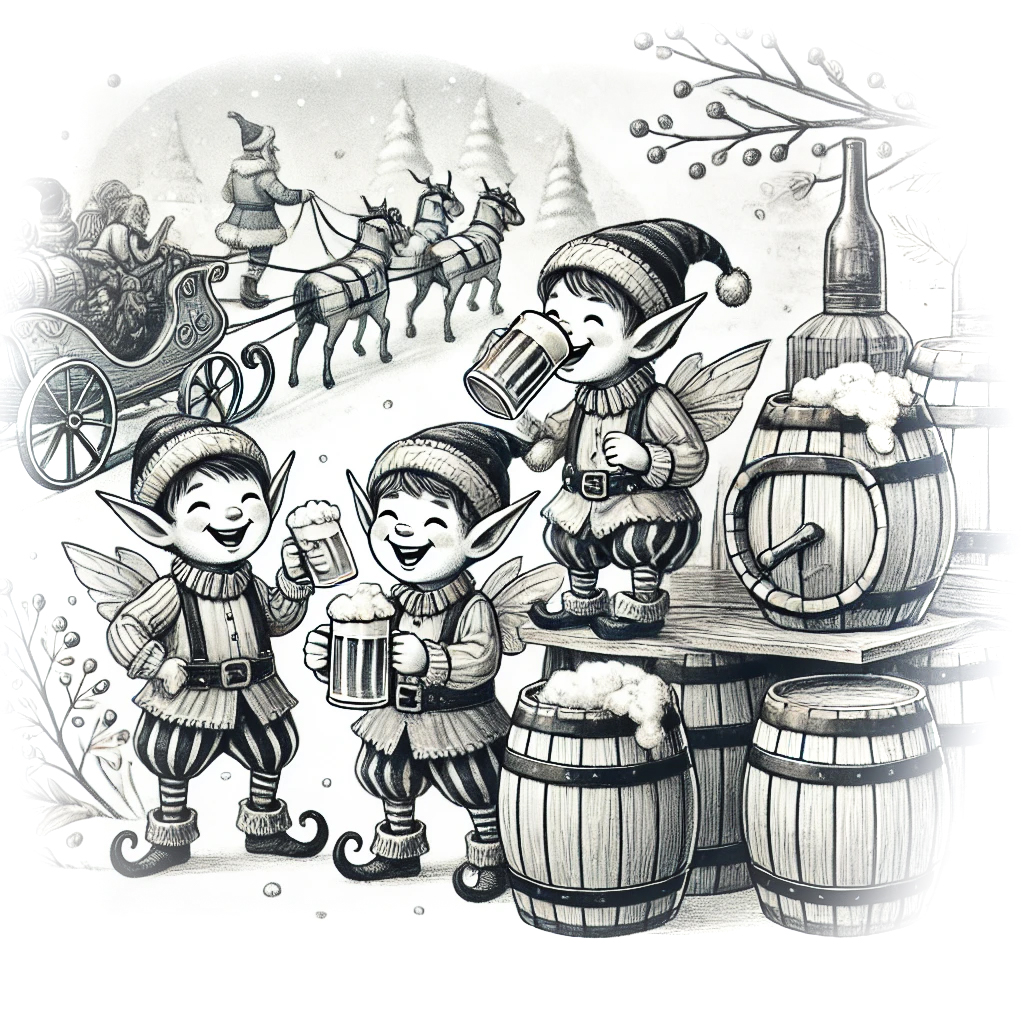
\includegraphics[width=0.6\textwidth]{elfy_zadanie_piwo.jpg} % Zmień "zdj.png" na nazwę pliku z obrazkiem
\end{center}

% Treść zadania
\noindent W browarze Świętego Mikołaja przechowywane jest $n$ beczek z piwem o podstawie o polu 1. Beczki są ustawione w rzędzie i każda z nich ma określoną wysokość $h[i]$. Drużyna transportowa natrafiła jednak na pewien problem. Otóż im wyższe sanie, tym większy koszt dostawy, zatem elfy naturalnie chcą użyć najniższych możliwych sań do transportu. Aby zmieścić daną beczkę na saniach, jej wysokość nie może przekraczać wysokości sań $H$, natomiast elfy mogą odpowiednio odciąć beczke od góry, żeby ta mogła się zmieścić (w wyniku tej operacji naturalnie zmienia sie jej objętość). Dodatkowo, elfy muszą zaspokoić niemałe zapotrzebowanie na napoje wyskokowe, które wynosi $V$.\\\\Wyznacz minimalną wartość $H$, dla której elfy będą w stanie zaspokoić zapotrzebowanie $V$, lub NIE jeśli taka wartość nie istnieje.


% Sekcja wejścia
\section*{Wejście}
Pierwszy wiersz wejścia zawiera dwie liczby całkowite $n$ i $V$ ($1 \leq n \leq 100\,000$), ($1 \leq V \leq \sum h[i]$) oznaczające ilość beczek w browarze oraz zapotrzebowanie na piwo.\\Kolejne $n$ wierszy zawiera po jednej liczbie całkowitej oznaczającej wysokość danej beczki $h[i]$, gdzie ($1 \leq h[i] \leq 10^9$).

% Sekcja wyjścia
\section*{Wyjście}
Wypisz jak najmniejszą wartość $H$, dla której spełnione jest wymagane zapotrzebowanie.
\newpage
% Sekcja przykładów
\section*{Przykład}
\begin{multicols}{2}
\noindent\textbf{Wejście:} \\
\exampleinput

\columnbreak

\noindent\textbf{Wyjście:} \\
\exampleoutput
\end{multicols}

\noindent Wyjaśnienie: \explanation

% Sekcja oceniania
\section*{Ocenianie}
Zestaw testów dzieli się na następujące podzadania:
\begin{center}
\subtasktable
\end{center}

% Stopka
\vspace*{\fill}
\noindent\rule{\textwidth}{0.4pt} \\
\small \textbf{Autor:} Filip Nowak \hfill \textbf{VIII LO im. Władysława IV w Warszawie}

% Komentarze:
% W polu \tasktitle wpisz pełny tytuł zadania.
% W polu \taskshort wpisz skrócony tytuł zadania.
% W polu \contestinfo wpisz informacje o konkursie.
% W polu \memorylimit wpisz limit pamięci.
% W polach \exampleinput i \exampleoutput wpisz dane przykładowe wejścia i wyjścia.
% W polu \explanation wpisz wyjaśnienie przykładu.
% W polu \subtasktable wpisz tabelę z podzadaniami, ich ograniczeniami i punktami.
% W stopce wstaw autora i nazwę szkoły.
\end{document}
